\documentclass[11pt]{article}

\usepackage{fullpage}
\usepackage{rotating}   
\usepackage{amsmath}
\usepackage{amssymb}
\usepackage{amsthm}
\usepackage{fancyhdr}
\usepackage{algorithm}
\usepackage{algorithmic}
\usepackage{bm}
\usepackage{listings}
\usepackage{graphicx}
\usepackage{caption2}
\usepackage{subfigure}
\usepackage{float}
\usepackage{extpfeil}
\usepackage{color}
\usepackage[usenames,dvipsnames]{xcolor}


\newtheorem{theorem}{Theorem}[section]
\newtheorem{lemma}[theorem]{Lemma}
\newtheorem{corollary}[theorem]{Corollary}
\newtheorem{proposition}[theorem]{Proposition}
\newtheorem{definition}[theorem]{Definition}
\newtheorem{conjecture}[theorem]{Conjecture}
\newtheorem{remark}[subsection]{Remark}

%%
\newcommand\numberthis{\addtocounter{equation}{1}\tag{\theequation}}

%% define new symbols
\def\bx{\bm{x}}
\def\bb{\bm{b}}
\def\ba{\bm{a}}
\def\bc{\bm{c}}
\def\bf{\bm{f}}
\def\by{\bm{y}}
\def\bu{\bm{u}}
\def\bv{\bm{v}}
\def\BW{\bm{W}}
\def\BA{\bm{A}}
\def\bz{\bm{z}}
\def\BZ{\bm{Z}}
\def\BH{\bm{H}}
\def\BL{\bm{L}}
\def\BU{\bm{U}}
\def\BV{\bm{V}}
\def\BB{\bm{B}}
\def\BC{\bm{C}}
\def\BD{\bm{D}}
\def\BE{\bm{E}}
\def\BW{\bm{W}}
\def\BQ{\bm{Q}}
\def\BG{\bm{G}}
\def\BA{\bm{A}}
\def\BX{\bm{X}}
\def\BY{\bm{Y}}
\def\BQ{\bm{Q}}
\def\BI{\bm{I}}
\def\BR{\bm{R}}

%% define new brackets
\def\la{\left\langle}
\def\ra{\right\rangle}
\def\ln{\left\|}
\def\rn{\right\|}
\def\lb{\left(}
\def\rb{\right)}
\def\lsb{\left[}
\def\rsb{\right]}
\def\lcb{\left\{}
\def\rcb{\right\}}

%%
\DeclareMathOperator*{\argmin}{arg\,min}
\DeclareMathOperator*{\argmax}{arg\,max}

%%
\title{Homework VII}
\author{Name: Shao Yanjun, Number: 19307110036}


\begin{document}
\maketitle

%------------------------------------
\begin{abstract}
This is Daniel's homework of  "Numerical Algorithms with Case Studies II".
\end{abstract}
%-------------------------------------
%=====================
\section{Problems}
\paragraph{Q1}
We calculate the integral first (eliminate the constant because it's useless)
\begin{align}
	r(a,b,c)=\int_{0}^{\frac{\pi}{2}}|sin(x)-ax^2-bx-c|^2dx&=	\int_{0}^{\frac{\pi}{2}}sin^2(x)-2(ax^2-bx-c)sin(x)+(ax^2-bx-c)^2dx\\
	&=-(4a-2c)cos(x)-2bsin(x)+2bxcosx-4axsin(x)+2ax^2cosx\\
	&+c^2x + x^3(b^2/3 + (2ac)/3) + (a^2*x^5)/5 + (abx^4)/2 + bcx^2\bigg|^{\frac{\pi}{2}}_0\\
	&=4a - 2b - 2c - 2\pi a + \frac{\pi}{2} c^2 + \frac{\pi^3}{24}(b^2 + 2ac) + \frac{\pi^5}{160}a^2 + \frac{\pi^4}{32}ab + \frac{\pi^2}{4}bc	
\end{align}
Find derivative of $r(a,b,c)$,
\begin{equation}
	\left\{
	\begin{aligned}
		r'_a(a,b,c)&=\frac{\pi^4}{32}a+\frac{\pi^3}{12}b+\frac{\pi^2}{4}c-2=0\\
		r'_b(a,b,c)&=\frac{\pi^5}{80}a+\frac{\pi^4}{32}b+\frac{\pi^3}{12}c+4-2\pi=0\\
		r'_c(a,b,c)&=\frac{\pi^3}{12}a+\frac{\pi^2}{4}b+\pi c-2=0		
	\end{aligned}
	\right.
\end{equation}
And the solution is $a=240\pi^{-3} + 2880\pi^{-4} - 11520\pi^{-5}$, $b=-144\pi^{-2} - 1344\pi^{-3} + 5760\pi^{-4}$ and $c=18\pi^{-1} + 96\pi^{-2} - 480\pi^{-3}$. The minimum value is $7.105584603731387$.
\paragraph{Q2}
We will approximate $x^3$ with a line, which means there are 3 alternation points. $r(x)=x^3+ax+b$
\begin{equation}
	\left\{
	\begin{aligned}
		r(-1)&=-1-a+b=8+2a+b=r(2)\\
		r'(x_1)&=3x_1^2+a=0\\
		r(x_1)&=x_1^3+ax_1+b=1+a-b=-r(-1)		
	\end{aligned}
	\right.
\end{equation}
The solution is $a=-3$ and $b=0$. The optimal value is $14$. 
\paragraph{Q3}
Use Remez's method, examine $|ln(1+x)+ax^2+bx+c|$ for several iterations. It converges very quickly, thanks to my good choice of the initial points. (All kinds of initial conditions produce fast convergence though...)
\begin{figure}[H]
	\centering
	\subfigure[iter=1]{
		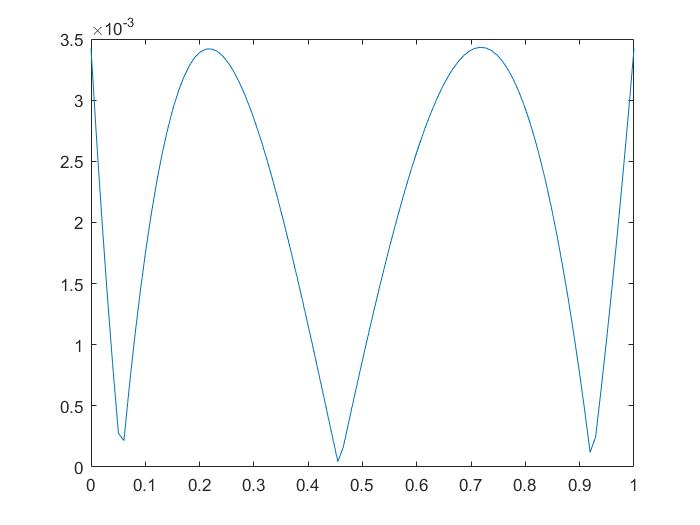
\includegraphics[width=0.4\linewidth]{remez_res_1.jpg}
	}
	\subfigure[iter=3]{
		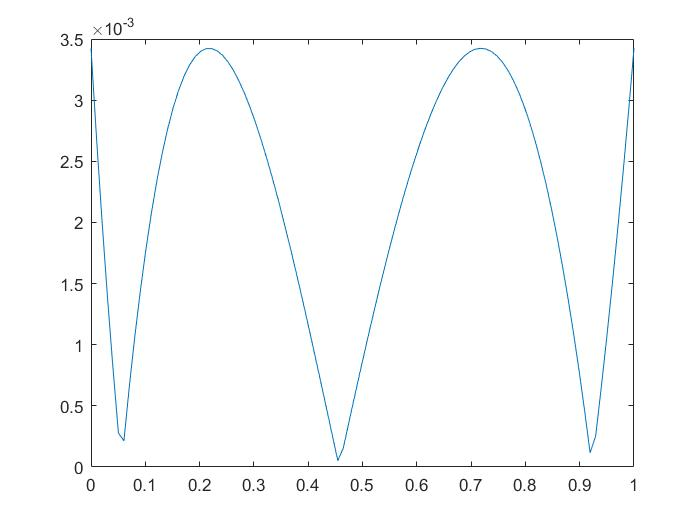
\includegraphics[width=0.4\linewidth]{remez_res_3.jpg}
	}
	\subfigure[iter=5]{
		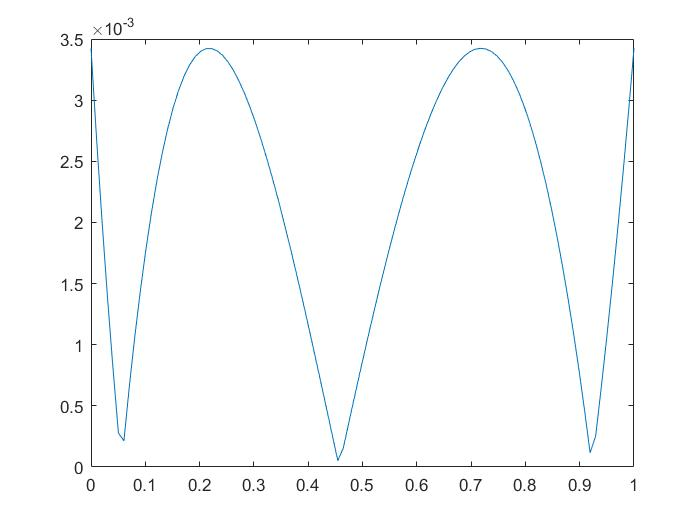
\includegraphics[width=0.4\linewidth]{remez_res_5.jpg}
	}
	\subfigure[iter=7]{
		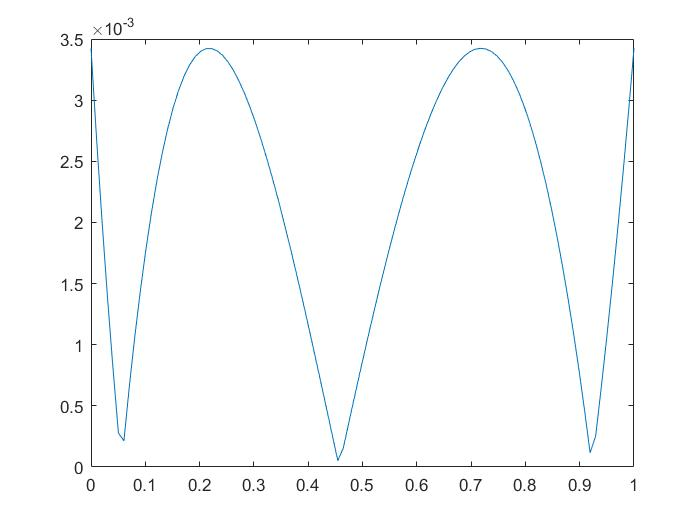
\includegraphics[width=0.4\linewidth]{remez_res_7.jpg}
	}
\end{figure}
And here is the comparison between the polynomial and the $f(x)$, and the best polynomial is $-0.239030719054479x^2+0.925329938214002x+0.003423980700211$. And the points should be chosen as $\{1,   0.718069281999180,0.217518624597682,0\}$
\begin{figure}[H]
	\centering
	\subfigure[approximation]{
		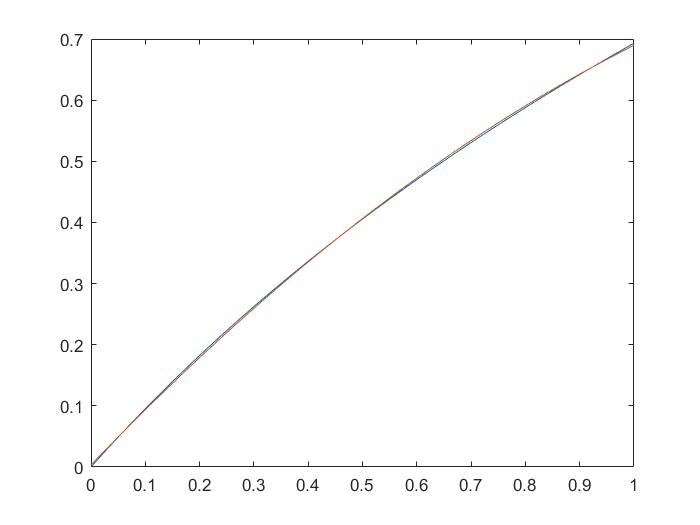
\includegraphics[width=0.4\linewidth]{remez_best.jpg}
	}
	\subfigure[residual]{
		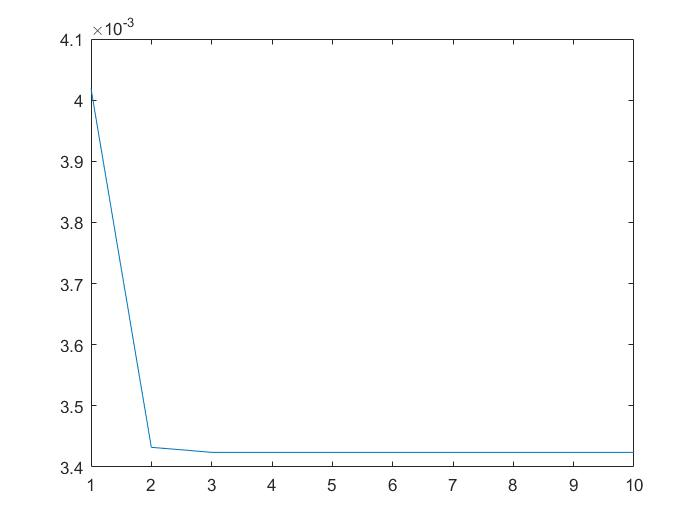
\includegraphics[width=0.4\linewidth]{remez_res.jpg}
	}
\end{figure}
\paragraph{Q4}
Do Taylor expansion of $f(x)=(1+x)^{-\frac{1}{2}}=1-\frac{1}{2}x+\frac{3}{8}x^2-\frac{16}{5}x^3+\frac{35}{128}x^4$. Solve the following linear systems and get an idea of Pade approximation,
\begin{align}
	\frac{ax+b}{cx+1}&=1-\frac{1}{2}x+\frac{3}{8}x^2\\
	\frac{ax^2+bx+c}{dx^2+ex+1}&=1-\frac{1}{2}x+\frac{3}{8}x^2-\frac{16}{5}x^3+\frac{35}{128}x^4
\end{align}
\qquad $p_1(x)=\frac{\frac{1}{4}x+1}{\frac{3}{4}x+1}$ and $p_2(x)=\frac{\frac{1}{16}x^2+\frac{3}{4}x+1}{\frac{5}{16}x^2+\frac{5}{4}+1}$. Check the polynomial vs $f(x)$
\begin{figure}[H]
	\centering
	\subfigure[pade approximation]{
		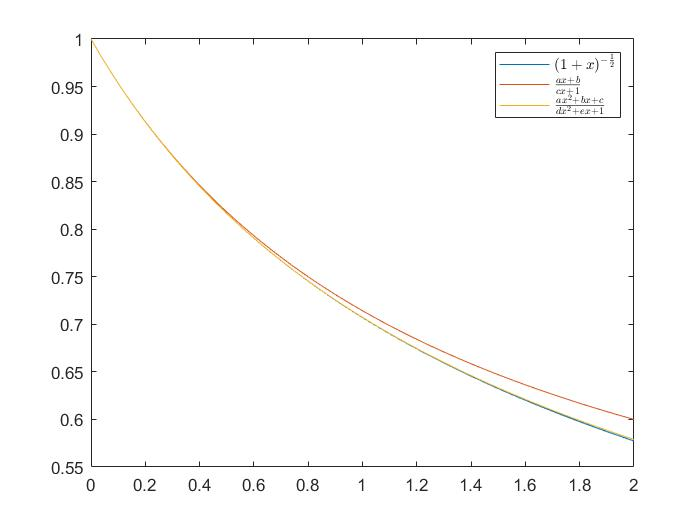
\includegraphics[width=0.4\linewidth]{pade_approx.jpg}
	}
	\subfigure[pade error]{
		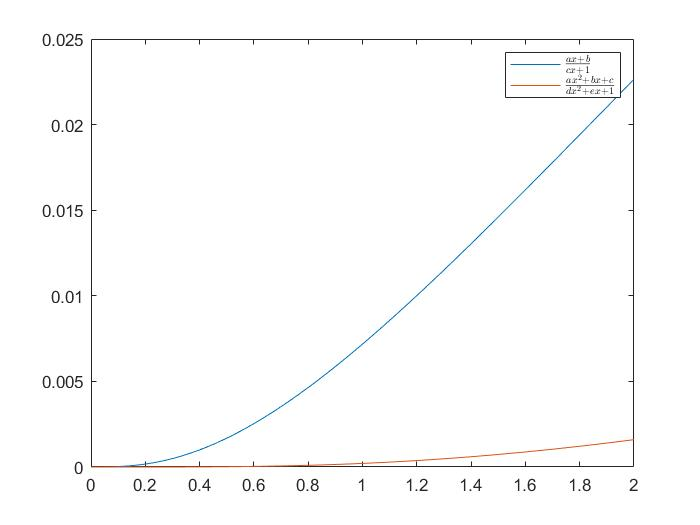
\includegraphics[width=0.4\linewidth]{pade_error.jpg}
	}
\end{figure}
%-------------------------------------
%=====================
\end{document}
